\section{Out-of-sample}
\begin{frame}{Out-of-sample}
\begin{table}[ht]
\center
\scalebox{0.6}{\begin{tabular}{lccccc}
\toprule
 & MAE & \(\text{R}^{\text{MAE}}\) && MSE & \(\text{R}^{\text{MSE}}\) \\ \midrule
 Benchmark model & 0.1111 & 1 && 0.0187 & 1 \\
AR\(\del{4}\) & 0.1312 & 1.1811 && 0.0272 & 1.454 \\  
Faktor model (IC\(_1\)) & 0.119 & 1.0717 && 0.0221 & 1.1798 \\
Lasso (CV) & 0.032 & 0.2877 && 0.0016 & 0.0876 \\
Lasso (BIC) & 0.0308 & 0.277 && 0.0015 & 0.0795 \\
Ridge regression (CV) & 0.0582 & 0.5239 && 0.0052 & 0.28 \\
Ridge regression (BIC) & 0.0573 & 0.5155 && 0.0051 & 0.2706 \\
Group lasso (CV) & 0.0352 & 0.3168 && 0.0019 & 0.1042  \\
Group lasso (BIC) & 0.0382 & 0.3437 && 0.0022 & 0.1202 \\
Adap. lasso m. OLS vægte (CV) & 0.0304 & 0.2733 && 0.0014 & 0.0729 \\
Adap. lasso m. OLS vægte (BIC) & 0.0310 & 0.2787 && 0.0014 & 0.0743 \\
Adap. lasso m. lasso vægte (CV) & $\mathbf{0.0298}$ & $\mathbf{0.2684}$ && $\mathbf{0.0013}$ & $\mathbf{0.0716}$ \\
Adap. lasso m. lasso vægte (BIC) & 0.0304 & 0.274  && 0.0014 & 0.0729 \\
Lasso$_{TG}$ (CV)& 0.0303 & 0.2724 && 0.0014 & 0.0744 \\ 
Lasso$_{TG}$ (BIC) & 0.031 & 0.279 && 0.0014 & 0.0767 \\
LARS (CV) &  0.0307 & 0.2761 && 0.0015 & 0.0802 \\
LARS (BIC) & 0.0305 & 0.2747 && 0.0015 & 0.0793 \\
Lasso LARS (CV) &  0.0352 & 0.317 && 0.002 & 0.1089 \\
Lasso LARS (BIC) & 0.0322 & 0.2901 && 0.0017 & 0.0903 \\
LARS$_{TG}$ (CV) & 0.0300 & 0.2701 && 0.0014 & 0.0745 \\
LARS$_{TG}$ (BIC) & 0.0301 & 0.2708 && 0.0014 & 0.0750 \\ \bottomrule
\end{tabular}}
\caption{Den gennemsnitlige absolutte og kvadrerede fejl samt gennemsnitlig tabs ratio mellem hver model og benchmark modellen.} \label{tab:mae_mse_vurdering}
\end{table}
\end{frame}

\begin{frame}{Out-of-sample}
\begin{figure}
 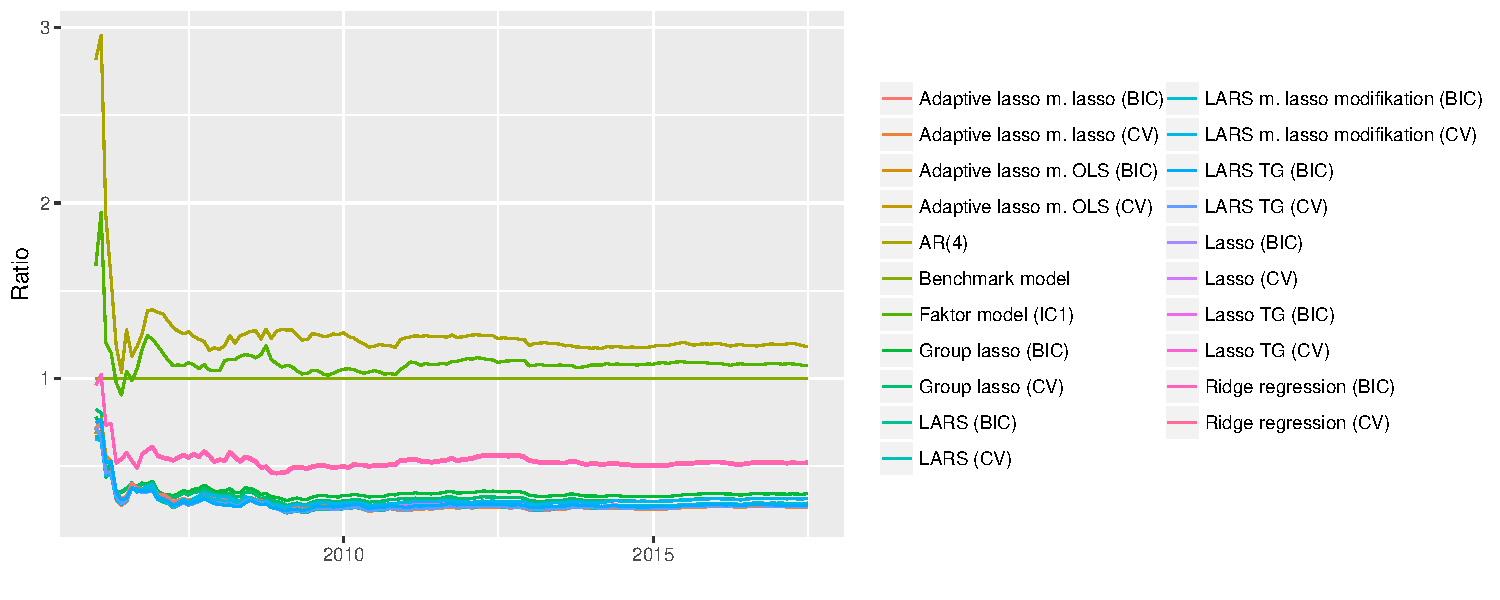
\includegraphics[width=1\linewidth, height=0.7\textheight]{slides/rolling_mae.pdf}
 \caption{Rullende gennemsnitlig absolut tabs ratio.}
 \end{figure}
\end{frame}

\begin{frame}{Out-of-sample}{Diebold-Mariano testen}
\begin{table}[ht]
\center
\scalebox{0.6}{\begin{tabular}{lcc}
\toprule
% & \(\abs{y_t - \widehat{y}_{i,t}}\) & \(\del{y_t - \widehat{y}_{i,t}}^2\) \\ \midrule
 & Absolutte fejl & Kvadrerede fejl \\ \midrule
AR\(\del{4}\) & 0.0021 & 0.0032 \\  
Faktor model (IC\(_1\)) & 0.1692 & 0.1183 \\
Lasso (CV) & 0 & $2.933\cdot 10^{-12}$ \\
Lasso (BIC) & 0 & $2.728\cdot 10^{-12}$ \\
Ridge regression (CV) & $6.418 \cdot 10^{-13}$  & $3.551\cdot 10^{-9}$  \\
Ridge regression (BIC) &$2.85\cdot 10^{-13}$& $2.507\cdot 10^{-9}$\\
Group lasso (CV) & 0 &$ 5.999\cdot 10^{-12}$  \\
Group lasso (BIC) & 0& $8.845\cdot 10^{-12}$ \\
Adap. lasso m. OLS vægte (CV) & 0& $2.797\cdot 10^{-12} $\\
Adap. lasso m. OLS vægte (BIC) & 0& $2.905\cdot 10^{-12}$\\
Adap. lasso m. lasso vægte (CV) & 0 & $2.676\cdot 10^{-12}$\\
Adap. lasso m. lasso vægte (BIC) & 0& $2.814\cdot 10^{-12}$\\
Lasso$_{TG}$ (CV)&  0 & 0 \\
Lasso$_{TG}$ (BIC) & 0 & 0 \\
LARS (CV) & 0 & $2.64\cdot 10^{-12}$  \\
LARS (BIC) & 0& $2.615\cdot 10^{-12}$ \\
Lasso LARS (CV) & 0& $4.694 \cdot 10^{-12}$ \\
Lasso LARS (BIC) & 0& $3.328 \cdot 10^{-12}$ \\ 
LARS$_{TG}$ (CV) & 0 & 0 \\
LARS$_{TG}$ (BIC) &0 & 0\\ \bottomrule
\end{tabular}}
\caption{\(p\)-værdier for Diebold-Mariano testen for hver model imod benchmark modellen.
\(p\)-værdier \(< 2.2 \cdot 10^{-16}\) sættes til 0.}
\end{table}
\end{frame}

\begin{frame}{Out-of-sample}{MCS}
\begin{table}[ht]
\center
\scalebox{0.6}{\begin{tabular}{lllll}
\toprule
%\multicolumn{4}{c}{\(\abs{y_t - \widehat{y}_{i,t}}\) } & \multicolumn{4}{c}{\(\del{y_t - \widehat{y}_{i,t}}^2\)} \\
\multicolumn{2}{c}{\(\text{T}_\text{R}\)} & & \multicolumn{2}{c}{\(\text{T}_\text{max}\)} \\
\cmidrule{1-2} \cmidrule{4-5} 
\(\alpha = 0.1\) & \(\alpha = 0.2\) & & \(\alpha = 0.1\) & \(\alpha = 0.2\) \\ \midrule
Benchmark model & Benchmark model  && Benchmark model  & Benchmark model \\
AR\((4)\) & AR\((4)\) && AR\((4)\) & AR\((4)\) \\
Lasso (CV) & Lasso (CV) && Faktor (IC\(_1\)) & Lasso (CV) \\
Lasso (BIC) & Lasso (BIC) && Lasso (CV) & Lasso (BIC) \\
Group lasso (CV) & Group lasso (CV) && Lasso (BIC) & Ridge regression (CV) \\
Group lasso (BIC) & Group lasso (BIC) && Ridge regression (CV) & Ridge regression (BIC) \\
Adap. lasso m. OLS vægte (CV) & Adap. lasso m. OLS vægte (CV) && Ridge regression (BIC) & Group lasso (CV) \\
Adap. lasso m. OLS vægte (BIC) & Adap. lasso m. OLS vægte (BIC) && Group lasso (CV) & Group lasso (BIC) \\
Adap. lasso m. lasso vægte (CV) & Adap. lasso m. lasso vægte (CV) && Group lasso (BIC) & Adap. lasso m. OLS vægte (CV) \\
Adap. lasso m. lasso vægte (BIC) & Adap. lasso m. lasso vægte (BIC) && Adap. lasso m. OLS vægte (CV) & Adap. lasso m. OLS vægte (BIC) \\
Lasso\(_{TG}\) (BIC) & Lasso\(_{TG}\) (BIC) && Adap. lasso m. OLS vægte (BIC) &  Adap. lasso m. lasso vægte (CV)  \\
LARS (CV) & LARS (CV) && Adap. lasso m. lasso vægte (CV) & Adap. lasso m. lasso vægte (BIC) \\
LARS (BIC) & LARS (BIC) && Adap. lasso m. lasso vægte (BIC) & Lasso\(_{TG}\) (CV) \\
Lasso LARS (CV) & Lasso LARS (CV) &&  Lasso\(_{TG}\) (CV) &  Lasso\(_{TG}\) (BIC) \\
Lasso LARS (BIC) & Lasso LARS (BIC) && Lasso\(_{TG}\) (BIC)  & LARS (CV) \\
& && LARS (CV)& LARS (BIC) \\
& && LARS (BIC)& Lasso LARS (CV) \\
& && Lasso LARS (CV) & Lasso LARS (BIC) \\
& && Lasso LARS (BIC) & LARS\(_{TG}\) (CV) \\ 
& && LARS\(_{TG}\) (CV) & LARS\(_{TG}\) (BIC) \\ 
& && LARS\(_{TG}\) (BIC) &  \\ \bottomrule
\end{tabular}}
\caption{80\% og 90\% model confidence set for arbejdsløshedsraten for absolutte og kvadrerede fejl.} \label{tab:mcs_tab}
\end{table}
\end{frame}


%%% Local Variables:
%%% mode: latex
%%% TeX-master: "../beamer"
%%% End:
